\documentclass[11pt]{article}
\usepackage{amssymb}
\usepackage{amsthm}
\usepackage{enumitem}
\usepackage{physics,amsmath}
\usepackage{bm}
\usepackage{adjustbox}
\usepackage{mathrsfs}
\usepackage{graphicx}
\usepackage{siunitx}
\usepackage[mathscr]{euscript}

\title{\textbf{Solved selected problems of Classical Mechanics - Gregory}}
\author{Franco Zacco}
\date{}

\addtolength{\topmargin}{-3cm}
\addtolength{\textheight}{3cm}

\newcommand{\hatr}{\bm{\hat{r}}}
\newcommand{\hatx}{\bm{\hat{x}}}
\newcommand{\haty}{\bm{\hat{y}}}
\newcommand{\hatz}{\bm{\hat{z}}}
\newcommand{\hatth}{\bm{\hat{\theta}}}
\newcommand{\hatphi}{\bm{\hat{\phi}}}
\newcommand{\hatrho}{\bm{\hat{\rho}}}
\theoremstyle{definition}
\newtheorem*{solution*}{Solution}
\renewcommand*{\proofname}{\bf{Solution}}

\begin{document}
\maketitle
\thispagestyle{empty}

\section*{Chapter 13 - The Calculus of Variations and Hamilton's Principle}

\begin{proof}{\textbf{13.1}}
    By definition, extremals are solutions of the Euler-Lagrange equation.
    In this case $F = \dot x^2/t^3$ so we have that
    \begin{align*}
        \frac{\partial F}{\partial x} = 0 \quad\quad\quad
        \frac{\partial F}{\partial \dot x} = \frac{2\dot x}{t^3} 
    \end{align*}
    Hence the Euler-Lagrange equation takes the form
    \begin{align*}
        \frac{d}{dt}\bigg(\frac{2\dot x}{t^3}\bigg) - 0 &= 0\\
        \frac{2\ddot x}{t^3} - \frac{6\dot x}{t^4} &= 0\\
        \ddot x - \frac{3\dot x}{t} &= 0
    \end{align*}
    Now we solve the equation by setting $v = \dot x$ hence
    \begin{align*}
        \frac{dv}{dt} - \frac{3v}{t} &= 0\\
        \int\frac{dv}{3v} &= \int\frac{dt}{t}\\
        \frac{\log(v)}{3} &= \log(t) + C\\
        v &= Ct^3
    \end{align*}
    by replacing again and solving the equation we have that 
    \begin{align*}
        \frac{dx}{dt} &= Ct^3\\
        \int dx &= C\int t^3dt\\
        x &= Ct^4 + D
    \end{align*}
    The admissible extremals are those that satisfy the conditions
    $x(1) = 3$ and $x(2) = 18$ this way we find the values of
    $C = 1$ and $D = 2$ so the only admissible extremal of $J[x]$ is given by
    \begin{align*}
        \hat x &= t^4 + 2
    \end{align*}

    Finally, we want to show that this extremal provides
    a global minimum of $J[x]$. Let $h$ be any admissible variation and 
    consider the variation in $J$ that it produces
    \begin{align*}
        J[\hat x + h] - J[\hat x]
        &= \int_1^2 \frac{(4t^3 + \dot h)^2}{t^3} dt
        - \int_1^2 \frac{(4t^3)^2}{t^3} dt\\
        &= \int_1^2 16t^3 + 8\dot h + \frac{\dot h^2}{t^3} dt
        - \int_1^2 16t^3 dt\\
        &= 8 \bigg[h\bigg]_{t=1}^{t=2} + \int_1^2 \frac{\dot h^2}{t^3} dt\\
        &= \int_1^2 \frac{\dot h^2}{t^3} dt
    \end{align*}
    Where we used that $h$ is an admissible extremal hence it must satisfy
    $h(1) = h(2) = 0$. Since the integral of a positive function must be
    positive we see that
    \begin{align*}
        J[\hat x + h] - J[\hat x] = \int_1^2 \frac{\dot h^2}{t^3} dt \geq 0
    \end{align*}
    Thus $\hat x$ provides the global minimum of $J[x]$.
    The global minimum value of $J$ is therefore $J [t^4 + 2] = 60$. 

\end{proof}
\cleardoublepage
\begin{proof}{\textbf{13.3}}
    We want to find the extremals of the path functional
    \begin{align*}
        L[y] = \int_0^1 \sqrt{1 + \bigg(\frac{dy}{dx}\bigg)^2} dx
    \end{align*}
    By definition, extremals are solutions of the Euler-Lagrange equation.
    In this case $F(y,\dot{y}) = \sqrt{1 + \dot{y}^2}$ so there is no explicit
    dependence on $x$ this implies that if we satisfy the equation
    \begin{align*}
        \dot{y}\frac{\partial F}{\partial\dot{y}} - F = C
    \end{align*}
    then we satisfy the Euler-Lagrange equation too, hence we have that
    \begin{align*}
        \dot{y}\frac{\dot{y}}{\sqrt{1 + \dot{y}^2}} - \sqrt{1 + \dot{y}^2} &= C\\
        \frac{\dot{y}^2 - 1 - \dot{y}^2}{\sqrt{1 + \dot{y}^2}} &= C\\
        \sqrt{1 + \dot{y}^2} &= -\frac{1}{C}\\
        \dot{y}^2 &= -1 + \frac{1}{C^2}\\
        \int y &= \frac{\sqrt{1-C^2}}{C^2} \int dx\\
        y &= \frac{\sqrt{1-C^2}}{C^2} x + D
    \end{align*}
    Where $D$ is a constant of integration. Now applying the given
    initial and end conditions we get that $C = 1$ and $D = 0$ so 
    the admissible extremal is
    \begin{align*}
        \hat y &= 0        
    \end{align*}
    But this is a constant solution so it may or may not be a solution to the
    Euler-Lagrange equation, we must check, hence we have that
    \begin{align*}
        \frac{d}{dt}\bigg(\frac{\partial F}{\partial \dot y}\bigg) - \frac{\partial F}{\partial y} = 0\\
        \frac{d}{dt}\bigg(\frac{\dot{y}}{\sqrt{1 + \dot{y}^2}}\bigg) - 0 = 0\\
        \frac{\ddot{y}}{(1 + \dot{y}^2)^{3/2}} = 0
    \end{align*}
    So $\hat y = 0$ is a solution to the Euler-Lagrange equation and therefore
    an extremal.
\cleardoublepage
    Finally, we want to check $\hat y$ provides a global minimum for $L$.
    Let $h$ be any admissible variation and consider the variation in $L$
    that it produces
    \begin{align*}
        L[\hat y + h]
        % - L[\hat y]
        &= \int_0^1 \sqrt{1 + (\dot{\hat y} + \dot h)^2} dx\\
        % - \int_0^1 \sqrt{1 + \dot{\hat y}^2} dx\\
        &= \int_0^1 \sqrt{1 + \dot h^2} dx
        % - \int_0^1 dx\\
        % &= \int_0^1 \sqrt{1 + \dot h^2} dx - 1\\
    \end{align*}
    Also, we know that
    $$\int_0^1 \sqrt{1 + \dot{\hat y}^2} dx = \int_0^1 dx = 1$$
    And we have that
    \begin{align*}
        \int_0^1 \sqrt{1 + \dot h^2} dx \geq 1 = \int_0^1 dx
    \end{align*}
    Therefore $\hat y$ provides a local minimum for $L$.
\end{proof}
\cleardoublepage
\begin{proof}{\textbf{13.5}}
    Let us analyze the following system
    \begin{center}
        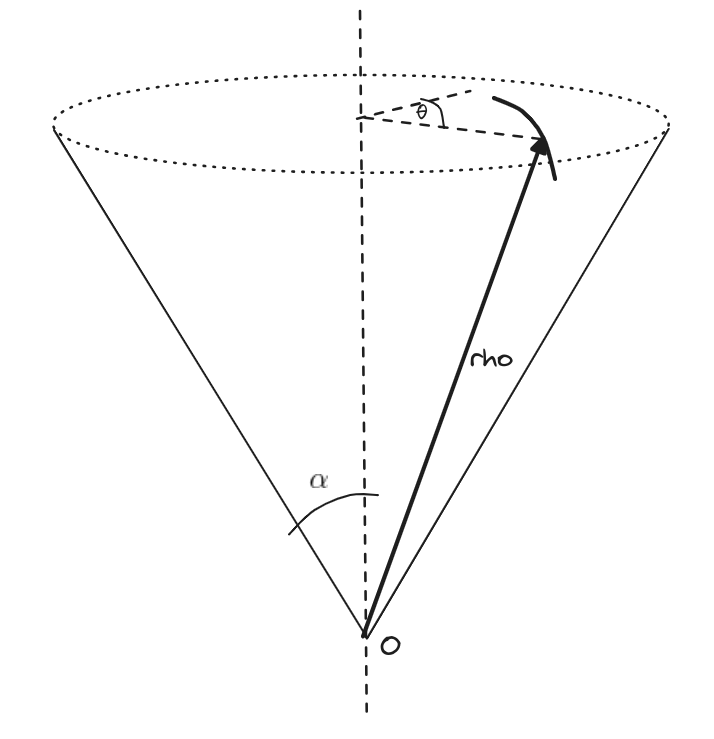
\includegraphics[scale=0.4]{ch13-5.png}
    \end{center}
    From this, we can write the differential length as
    \begin{align*}
        (ds)^2 = (d\rho)^2 + (\rho \sin\alpha d\theta)^2
    \end{align*}
    So integrating we get the length functional as follows
    \begin{align*}
        L = \int_{-\pi/2}^{\pi/2} ds =
        \int_{-\pi/2}^{\pi/2} \sqrt{\left(\frac{d\rho}{d\theta}\right)^2 + (\rho \sin\alpha)^2}~d\theta
    \end{align*}
    In this case, we have that
    $F(\rho,\dot{\rho}) = \sqrt{\dot\rho^2 + (\rho\sin\alpha)^2}$
    so there is no explicit dependence on $\theta$ this implies that if we
    satisfy the equation
    \begin{align*}
        \dot{\rho}\frac{\partial F}{\partial\dot{\rho}} - F = C
    \end{align*}
    then we satisfy the Euler-Lagrange equation too, hence we have that
    \begin{align*}
        \dot{\rho}\frac{\dot{\rho}}{\sqrt{\dot\rho^2 + (\rho\sin\alpha)^2}}
        - \sqrt{\dot\rho^2 + (\rho\sin\alpha)^2} &= C\\
        \frac{\dot{\rho}^2 - \dot\rho^2 - (\rho\sin\alpha)^2}
        {\sqrt{\dot\rho^2 + (\rho\sin\alpha)^2}} &= C\\
        \sqrt{\dot\rho^2 + (\rho\sin\alpha)^2} &= -\frac{(\rho\sin\alpha)^2}{C}\\
        \dot\rho^2  &= - (\rho\sin\alpha)^2 + \frac{(\rho\sin\alpha)^4}{C^2}\\
        \frac{d\rho}{d\theta} &= (\rho\sin\alpha)\sqrt{\frac{(\rho\sin\alpha)^2}{C^2} - 1}\\
    \end{align*}
    Now  we can integrate the equation as follows
    \begin{align*}
        \int \frac{d\rho}{(\rho\sin\alpha)\sqrt{\frac{(\rho\sin\alpha)^2}{C^2} - 1}}
        &= \int d\theta\\
        \frac{\arctan(\sqrt{\frac{(\rho\sin\alpha)^2}{C^2} - 1})}{\sin\alpha}
        &= \theta + D\\
        \arctan(\sqrt{\frac{(\rho\sin\alpha)^2}{C^2} - 1})
        &= (\theta + D)\sin\alpha\\
        \frac{(\rho\sin\alpha)^2}{C^2} - 1
        &= \tan^2\left((\theta + D)\sin\alpha\right)\\
        \rho &= \frac{C}{\sin\alpha}
        \sqrt{\tan^2\left((\theta + D)\sin\alpha\right) + 1}\\
        \rho &= \frac{C}{\sin\alpha}\sec((\theta + D)\sin\alpha)
    \end{align*}
    This is the equation for the extremals of $L$.
    Now applying the given initial and end conditions we get that
    \begin{align*}
        a = \frac{C}{\sin\alpha}\sec(-(\pi/2 - D)\sin\alpha)
        &= \frac{C}{\sin\alpha}\sec((\pi/2 + D)\sin\alpha)
    \end{align*}
    which implies that $D = 0$ and $C$ is
    \begin{align*}
        C \sec\left(\frac{\pi\sin\alpha}{2}\right) &= a\sin\alpha\\
        C &= \frac{a\sin\alpha}{\sec\left(\frac{\pi\sin\alpha}{2}\right)}
    \end{align*}
    Replacing the values for $C$ and $D$ we get that the admissible extremal is
    \begin{align*}
        \rho &=
        \frac{a\sec(\theta\sin\alpha)}{\sec(\frac{\pi\sin\alpha}{2})}\\
        \rho &=
        \frac{a\cos(\frac{\pi\sin\alpha}{2})}{\cos(\theta\sin\alpha)}\\
    \end{align*}
    \cleardoublepage
    Finally, we want to verify that this extremal is the same as the shortest
    path that would be obtained by developing the cone onto a plane.
    If we develop the cone onto a plane, we get that the path is a vertical
    line in the plane as shown below
    \begin{center}
        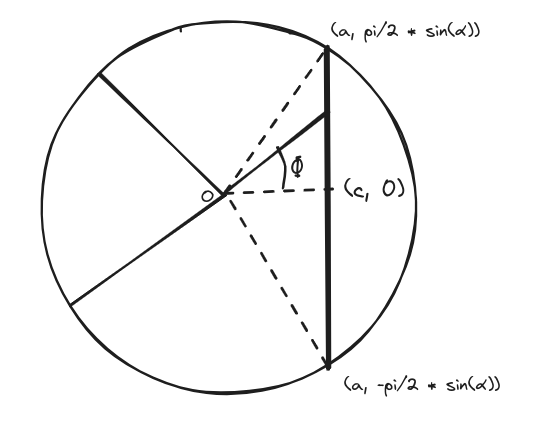
\includegraphics[scale=0.4]{ch13-5_1.png}
    \end{center}
    where the angle in the plane is given by $\phi = \theta \sin\alpha$.
    We know that the equation of a straight vertical line in polar coordinates
    is given by
    \begin{align*}
        \rho\cos(\phi) &= c
    \end{align*}
    where $c$ is the value of $\rho$ when $\phi = 0$ and from the drawing
    above we have that $\cos(\pi/2\sin(\alpha)) = c/a$ hence 
    \begin{align*}
        \rho\cos(\theta\sin\alpha) &= a\cos(\frac{\pi\sin(\alpha)}{2})
    \end{align*}
    Which is the admissible extremal that we have such that it satisfies
    the Euler-Lagrange equation.
\end{proof}
\end{document}






















